% !TEX encoding = UTF-8
% !TEX TS-program = pdflatex
% !TEX root = ../thesis.tex

\chapter{State of the art and technology background}
This chapter presents the pre-concepts needed to comprehend this paper's content fully.
As is understandable from the introduction, they are about Self-Sovereign Identity and 
blockchains. In addition, state of the art will be analyzed to see what has already been
done and what can be improved.
% /*//////////////////////////////////////////////////////////////
%                       TECHNOLOGY CONCEPTS
% //////////////////////////////////////////////////////////////*/
\section{Technology concepts}
This section will explain in detail SSI and blockchain technologies.
\subsection{Self-Sovereign Identity concepts}
Here can be read a brief reprise of what has already been saying about Self-Sovereign 
Identity and a description of its main primitives: VCs, VPs, and DIDs.
\subsubsection{Self-Sovereign Identity}
Self-Sovereign Identity is an approach to digital identity that gives individuals 
control over their data. SSI addresses the difficulty of establishing trust in 
interaction and allows people to interact in the digital world with the same freedom 
and ability to trust as they have in the offline world.
\vspace*{0.3cm}\\
To be trusted, a party in an interaction will present credentials to other parties, 
and those parties can verify that the credentials come from an \textbf{issuer} they trust.
This way, the \textbf{verifier}'s trust in the issuer is transferred to the credential 
\textbf{holder} (or \textbf{prover}). This basic structure of SSI with three participants 
is sometimes called the "triangle of trust.", simply because you need an element of trust
among these entities for them to work together.
\vspace*{0.3cm}\\
While this does not mean that there is a legal partnership or understanding between the 
entities involved, it does mean that each of the entities is willing to examine the 
credibility of the other, and this implicit trust is what constitutes this term.
\begin{center}
    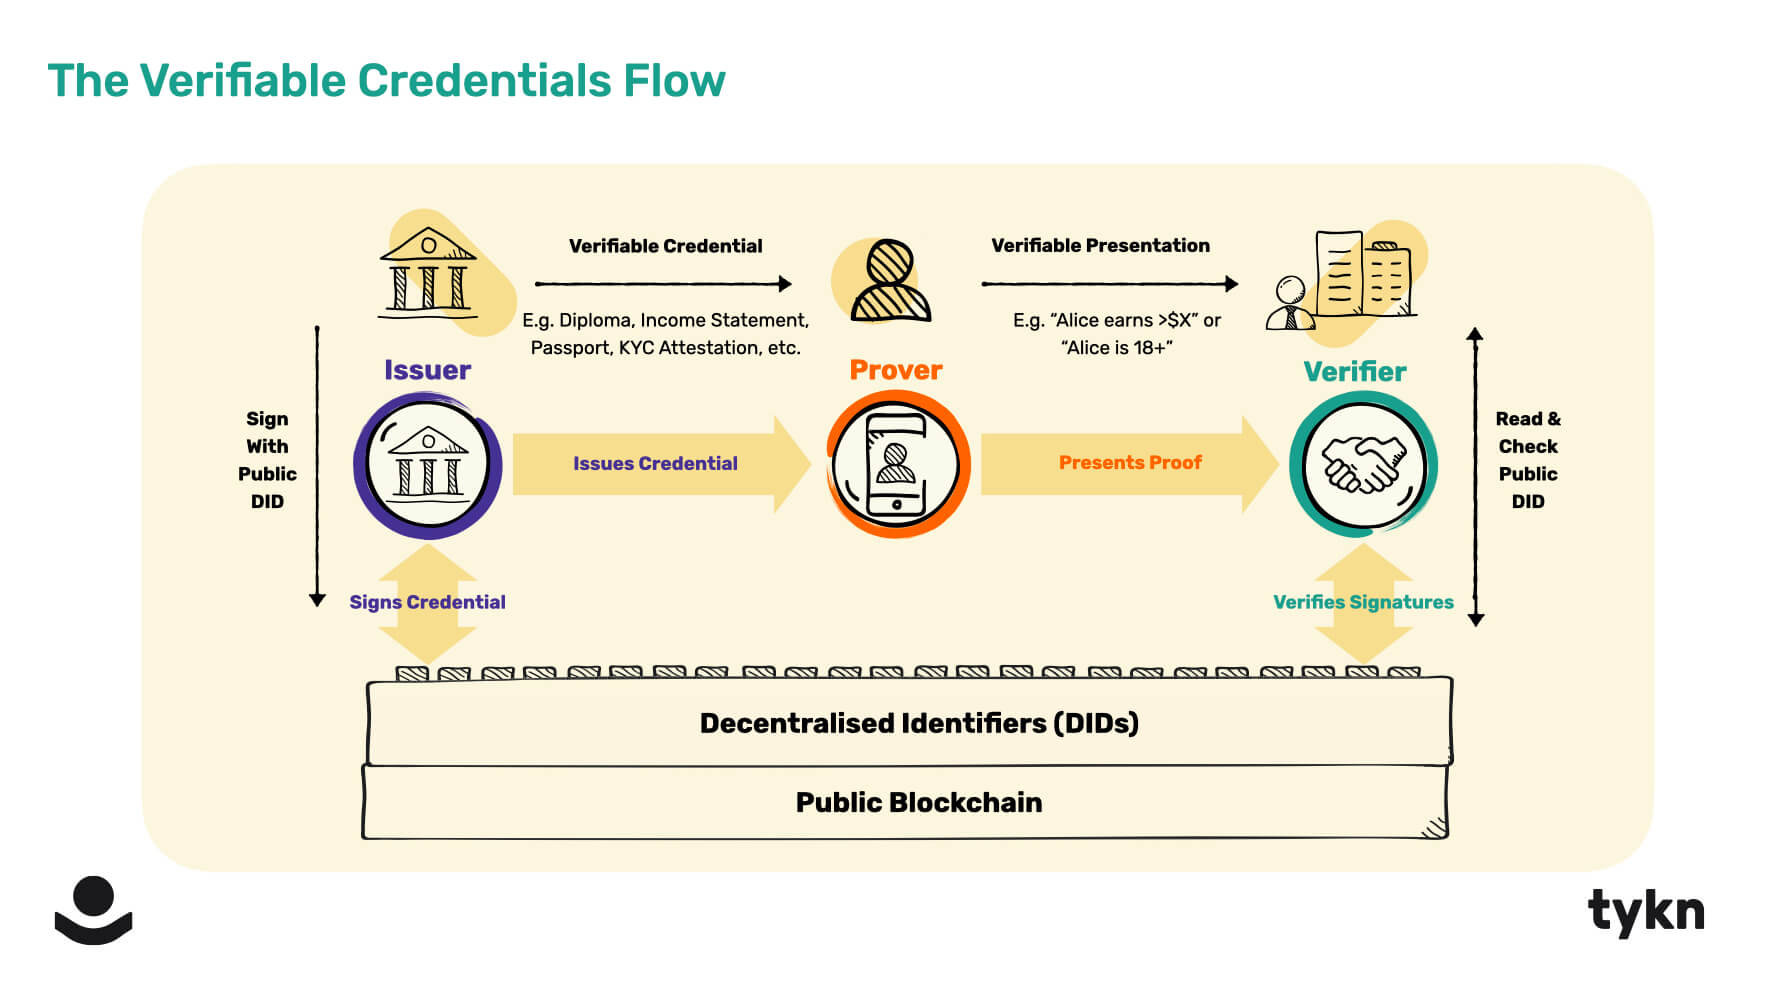
\includegraphics[scale=0.2]{chapter2/triangleTrust2.jpeg}
    \captionof{figure}{The triangle of trust: Prover, Issuer, and Verifier (by Tykn)}
\end{center}
\subsubsection{Verifiable Credential (VC)}
A verifiable credential can represent all of the same information that a physical 
credential represents. The addition of technologies, such as digital signatures, 
makes verifiable credentials more tamper-evident and more trustworthy than their 
physical counterparts.\\
\begin{center}
    \vspace*{-0.5cm}
    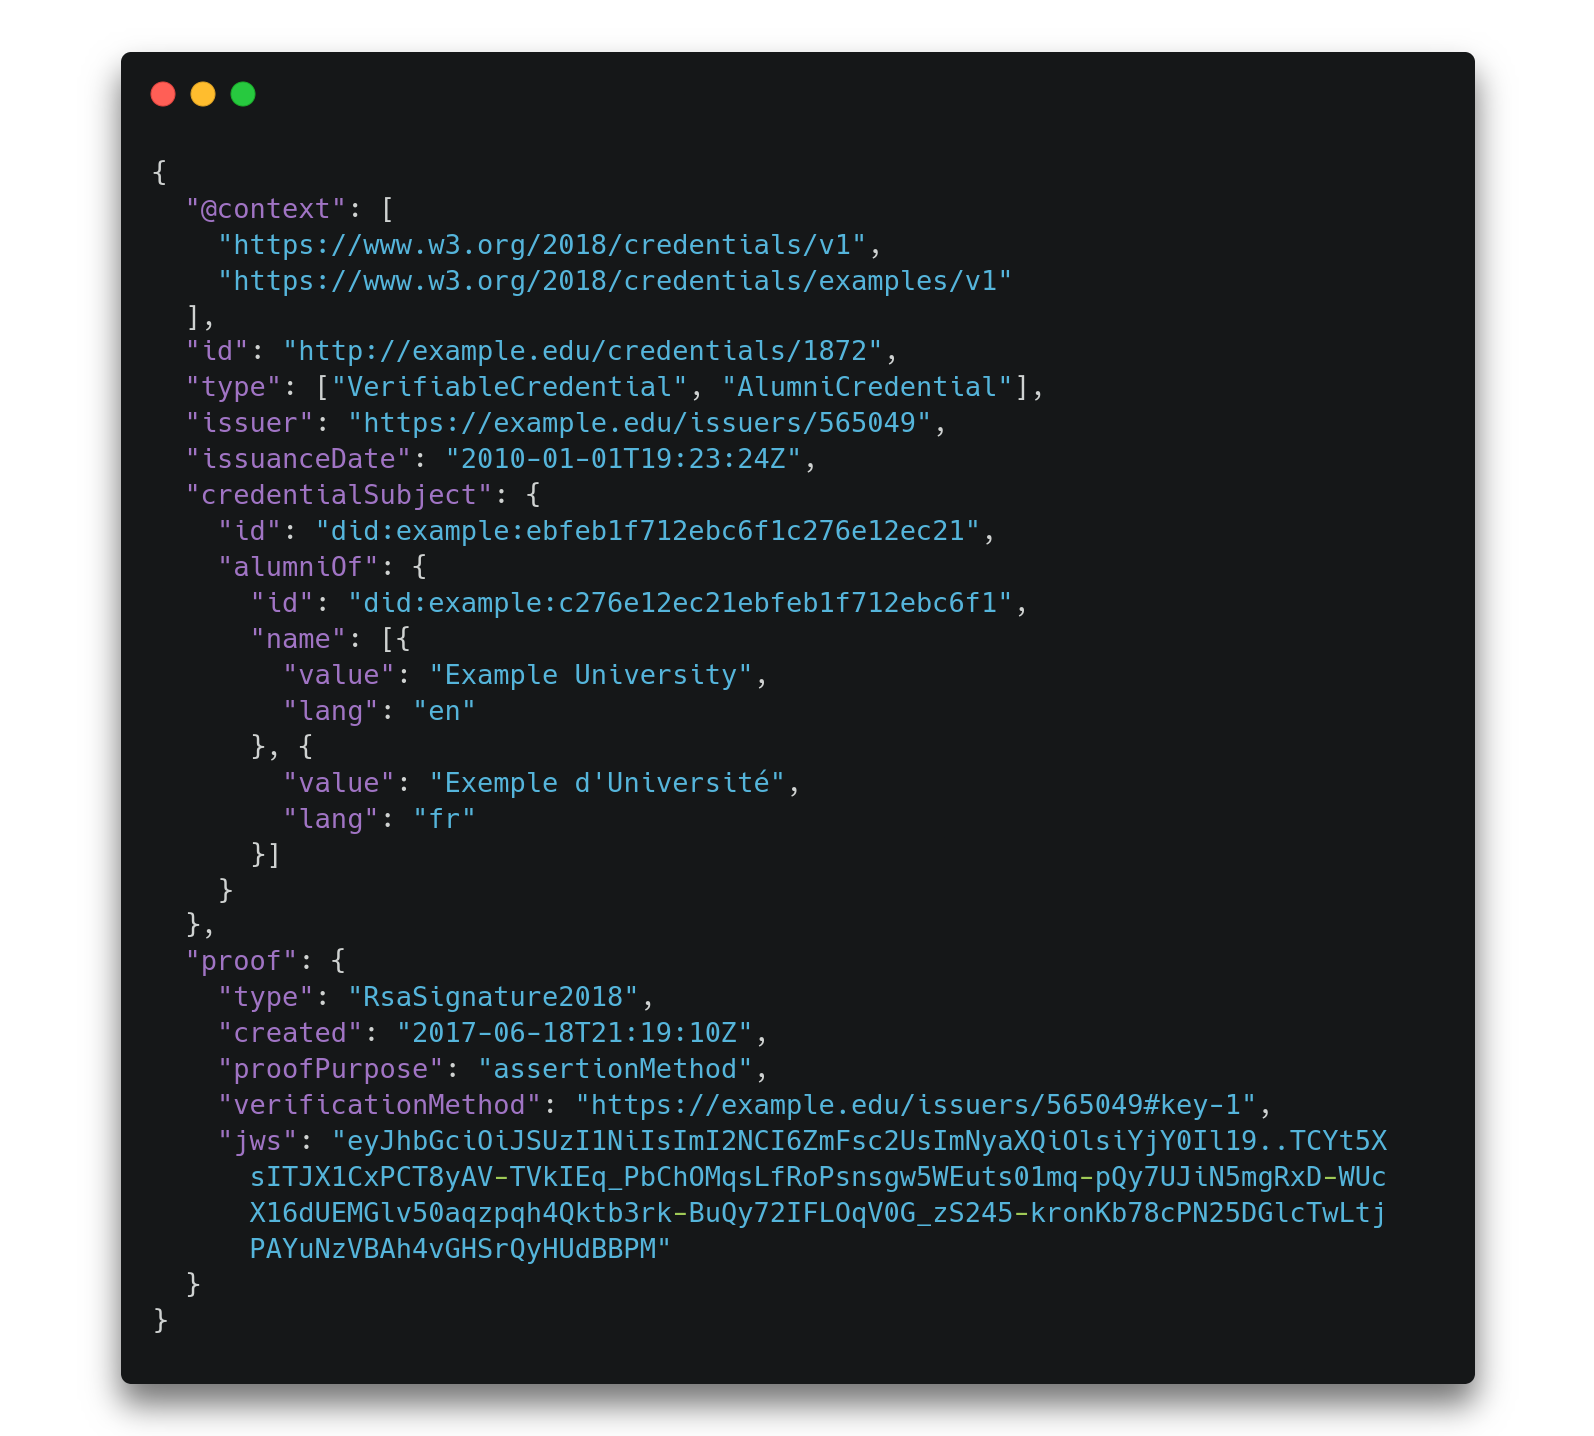
\includegraphics[scale=0.2]{chapter2/exampleVc.png}
    \captionof{figure}{Example of verifiable credential (VC)}
\end{center}
Holders of verifiable credentials can generate verifiable presentations and then share 
these verifiable presentations with verifiers to prove they possess verifiable 
credentials with certain characteristics.\\
Both verifiable credentials and verifiable presentations can be transmitted rapidly, 
making them more convenient than their physical counterparts when trying to establish 
trust at a distance.
The three main components of a VC are:
\begin{enumerate}
    \item \textbf{Metadata}: cryptographically signed by the issuer. It describes the credential
    properties, such as the issuer, the subject, the expiry date and time, a public key 
    to use for verification purposes, the revocation mechanism, and other information;
    \item \textbf{Claims}: a statement made about a subject. Example: “Janice`s date of 
    birth is 01/01/1990.”
    \item \textbf{Proofs}: a proof is data about the identity holder that allows others 
    to verify the source of the data (i.e., the issuer), check that the data belongs to 
    (only) the holder, that the data has not been tampered with, and finally, that the 
    issuer has not revoked the data.
\end{enumerate}

\subsubsection{Verifiable Presentation (VP)}
A verifiable presentation expresses data from one or more verifiable credentials and is 
packaged in such a way that the authorship of the data is verifiable. If verifiable 
credentials are presented directly, they become verifiable presentations. Data formats 
derived from verifiable credentials that are cryptographically verifiable but do not 
themselves contain verifiable credentials might also be verifiable presentations.
\begin{center}
    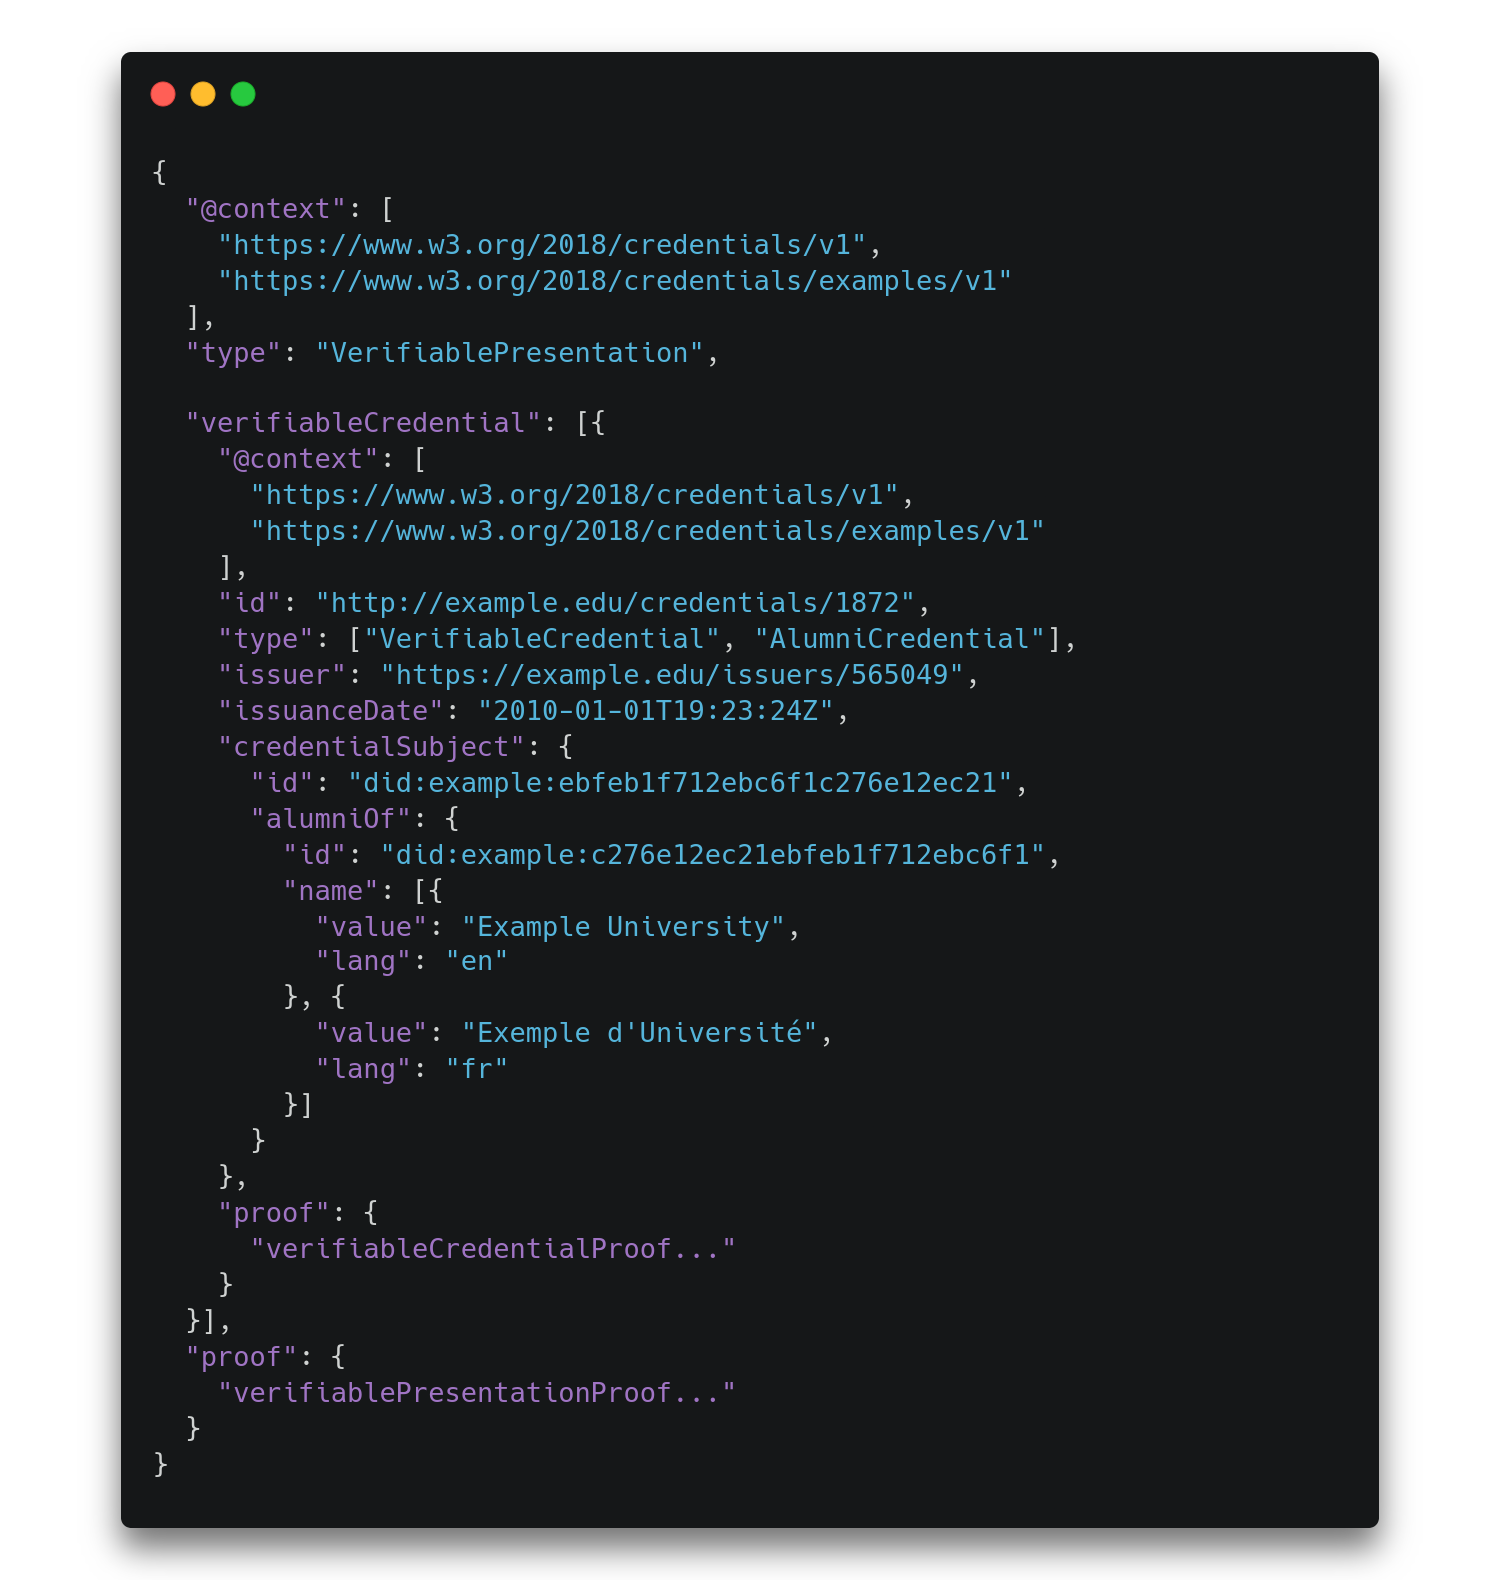
\includegraphics[scale=0.18]{chapter2/exampleVp.png}
    \captionof{figure}{Example of verifiable presentation (VP)}
\end{center}
The data in a presentation is often about the same subject but might have been issued by 
multiple issuers. The aggregation of this information typically expresses an aspect of 
a person, organization, or entity.

\subsubsection{Decentralized Identifier (DID)}
Decentralized identifiers are a new type of identifier that guarantees a verifiable, 
decentralized digital identity. A DID refers to any subject (e.g., a person, an 
organization, a data model, an abstract entity...).\\
DIDs are decoupled from centralized registries, identity providers, and certification 
authorities. Specifically, while other parties can be used to retrieve information 
about a DID, the design allows the controller of a DID to demonstrate control over it 
without requiring permission from other parties.
\begin{figure}[!htb]
    \begin{minipage}{0.48\textwidth}
      \centering
      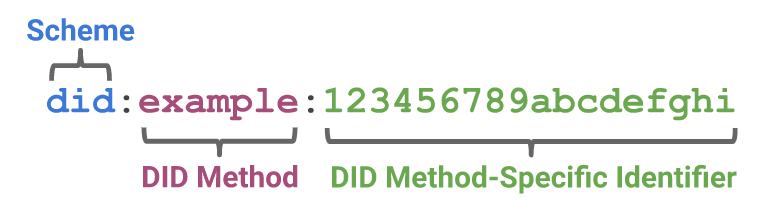
\includegraphics[width=1\linewidth]{chapter2/did1.png}
      \vspace{1.1cm}
      \caption{Example of a DID}
    \end{minipage}\hfill
    \begin{minipage}{0.48\textwidth}
      \centering
      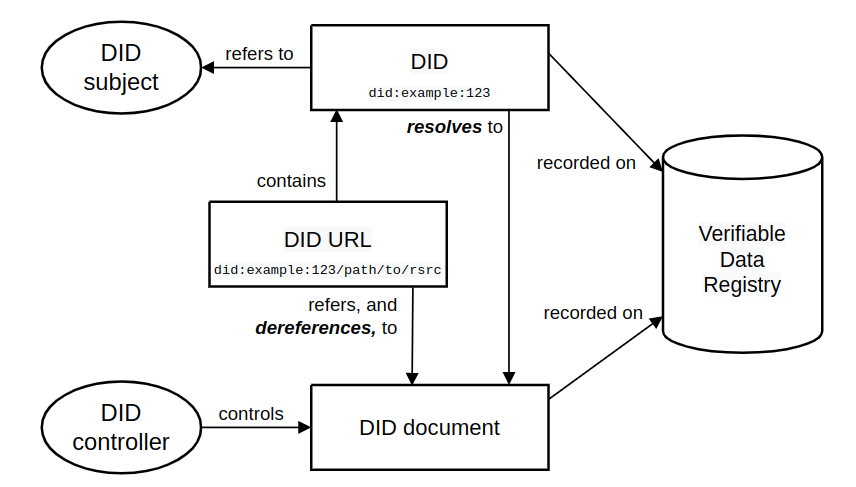
\includegraphics[width=1\linewidth]{chapter2/did2.png}
      \caption{DID architecture overview and basic components relationship}
    \end{minipage}
 \end{figure}
\begin{center}
    \vspace{-0.8cm}
    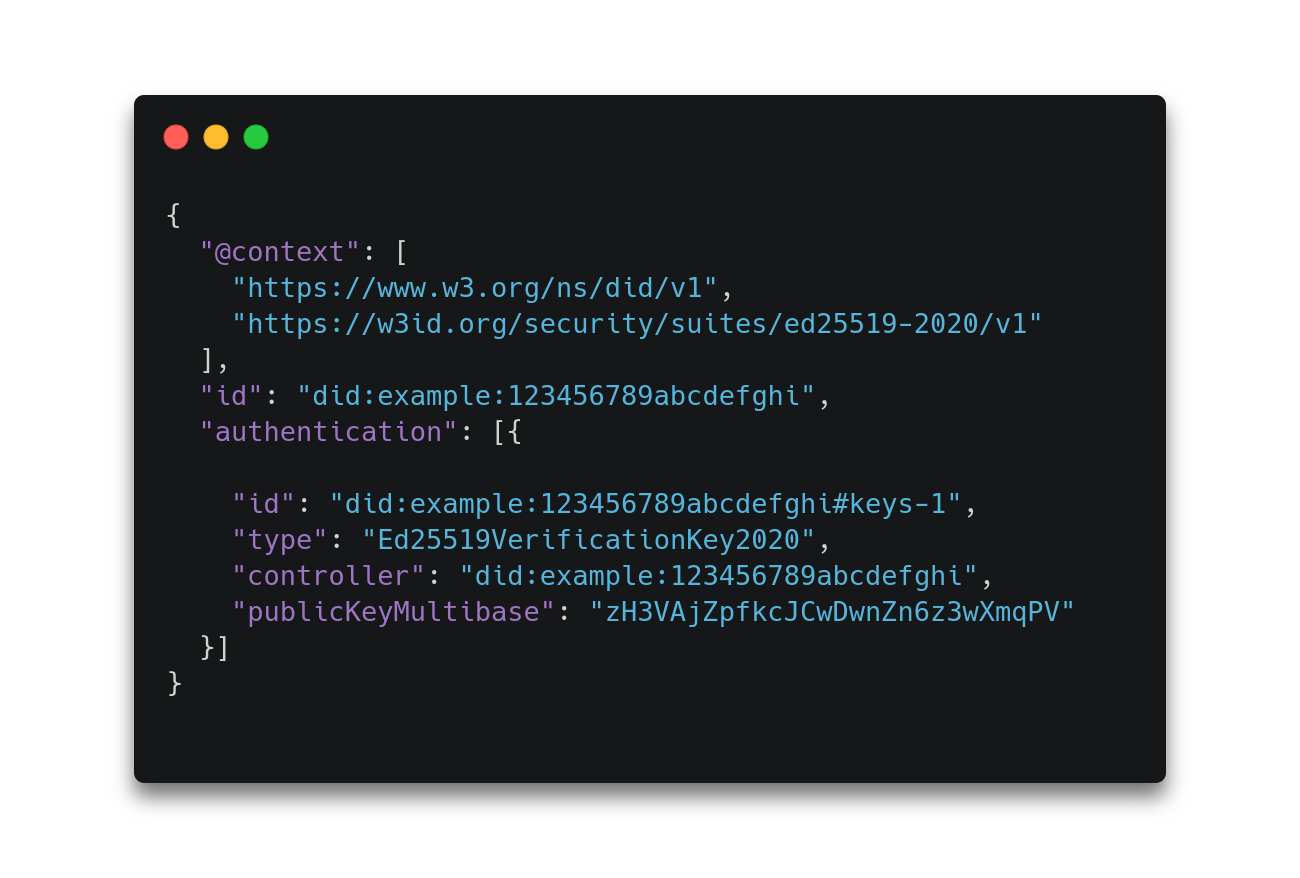
\includegraphics[scale=0.19]{chapter2/didDoc.png}
    \vspace{-0.4cm}
    \captionof{figure}{Example of DID document}
\end{center}
\vspace{0.5cm}
DIDs are Uniform Resource Identifiers (URIs) that associate a DID subject with a DID 
document that enables trusted interactions associated with that subject.
Each DID document may contain encrypted material, verification methods, or services, 
which provide a set of mechanisms that allow a DID controller to demonstrate control 
of the DID. Services enable trusted interactions associated with the subject of the 
DID. A DID may provide the means to return the DID subject itself if the DID subject 
is an information resource such as a data model.\\
A DID is a simple text string consisting of three parts: 1) the DID URI scheme 
identifier \footnote{The formal syntax of a decentralized identifier. The generic 
DID scheme begins with the prefix \textit{did:}.}, 2) the identifier for the DID method
\footnote{A definition of how a specific DID method scheme is implemented.}, and 3) 
the DID method-specific identifier.

\subsubsection{JavaScript Object Notation (JSON)}
The VC, VP and DID document code examples showed above are all in JSON.\\
The JSON is a lightweight data-interchange format. It is easy for humans to read and 
write, and for machines to parse and generate. It is based on a subset of the JavaScript
Programming Language Standard ECMA-262 3rd Edition - December 1999.\\
JSON is built on two structures:
\begin{itemize}
    \item A collection of name/value pairs. In various languages, this is realized as an 
    object, record, struct, dictionary, hash table, keyed list, or associative array.
    \item An ordered list of values. In most languages, this is realized as an array, 
    vector, list, or sequence.
\end{itemize}
These are universal data structures. Virtually all modern programming languages support 
them in one form or another. It makes sense that a data format that is interchangeable 
with programming languages also be based on these structures.
\subsection{Blockchain concepts}
Here we will introduce the main concepts of blockchain technology, essentials to 
understand the PoC development phase and some SDK features.
\subsubsection{Blockchain}
The blockchain is a shared, immutable database structured in the form of a chain of 
blocks, each of which contains a set of information. In essence, blockchains represent 
digital ledgers and perform different functions.
\begin{center}
    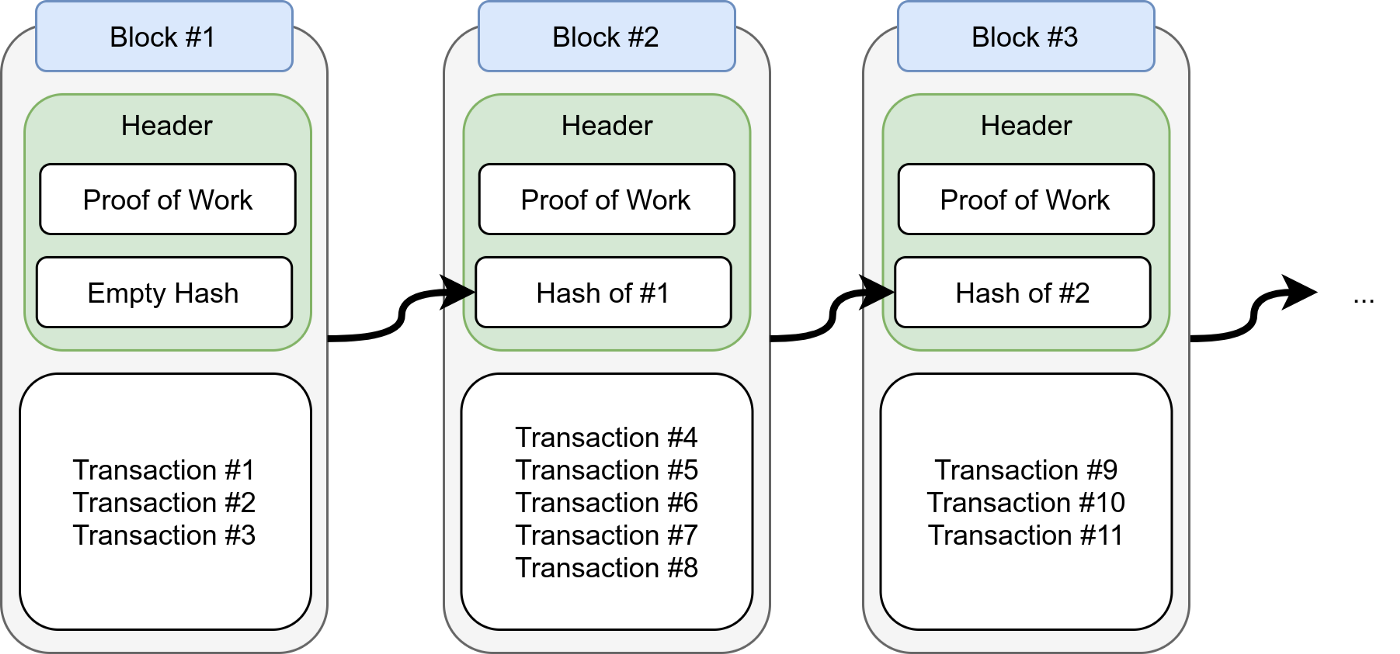
\includegraphics[scale=0.2]{chapter2/blockchain.png}
    \captionof{figure}{Simple blockchain visualization}
\end{center}
Physically it is composed of multiple \textbf{nodes}, i.e., computers that run the software 
(Client) of the blockchain. When a user wants to interact with the blockchain, he 
sends a \textbf{transaction} to one of the nodes. This transaction will then reach a pool with 
all the transactions in the pending state, and the nodes that are dealing with the 
consensus part will take care of updating the state of the blockchain by inserting 
several transactions (meeting certain conditions) within the new \textbf{block} that will
be added to the chain.\\
Its main features are data digitalization, decentralization, disintermediation, 
transfer traceability and programmability, transparency/verifiability, and immutability.
\subsubsection{Permissionless and permissioned blockchains}
We can divide blockchains into two main categories: permissionless and permissioned.
This division is based on the access to the network.
\begin{itemize}
    \item \textbf{Permissionless blockchains} are the most popular model. As its name implies, these 
    networks allow access to anyone and are decentralized and public. Consequently, 
    everyone can run a node or connect to the blockchain.\\
    This accessibility implies a trade-off on speed; these networks are often slower than 
    their permissioned counterparts, with fewer members, and transactions are validated by 
    everyone running a connected node. The primary consensus mechanisms are Proof-of-Work 
    (PoW) and Proof-of-Stake (PoS) \footnote{PoW involves hashing (mining) power, PoS voting 
    (using blockchain coins) power, through validator nodes.}.\\
    What is of most interest in this scenario is that in a permissionless blockchain, 
    everyone can interact, and data is public, so \textbf{preserving privacy becomes difficult}.
    \item \textbf{Permissioned blockchains} are private networks that require permission to
    join. They are usually run by a single organization or a consortium of organizations.\\
    The main advantage of permissioned blockchains is speed. They are faster than
    permissionless blockchains because they have fewer members and transactions are
    validated by a smaller number of nodes. The main consensus mechanisms are Raft and 
    Practical Byzantine Fault Tolerance (PBFT).\\
    The main peculiarity of permissioned blockchains is that they are not decentralized
    and are not public. This means that only a limited number of people can interact with
    the blockchain, and data is not public, so \textbf{privacy can be preserved}.
\end{itemize}

\subsubsection{Ethereum}
Ethereum is a permissionless blockchain, i.e., open to anyone who wants to interact 
with it: the trade-off is the introduction of fees, to be paid every time anyone wants 
to change the state of the Ethereum Virtual Machine (EVM), to mitigate the problems 
that the permissionless factor introduces (e.g., transaction spam). In the read-only 
case, no fee needs to be paid. Anyone can then view what is happening in the blockchain 
and, more importantly, use it. To do so, a user has to generate a \textbf{wallet} (i.e.,
an address in the blockchain), transfer some funds to it from outside \footnote{Usually
from a centralized exchange, where cryptoc-urrencies can be traded for fiat currencies
like EUR or USD, or from another blockchain.} so that fees can be paid, and start 
interacting with the decentralized applications that are already developed or transfer 
funds to other wallets. In fact, one of the main features of Ethereum is \textbf{smart 
contracts}: they are programs that run on the Ethereum blockchain. They are a collection 
of code (functions) and data (state) that resides at a specific address on the 
Ethereum blockchain.
\subsubsection{Hyperledger}
Hyperledger Foundation is a nonprofit organization that combines all the resources and 
infrastructure needed to ensure thriving and stable ecosystems around open-source 
software blockchain projects.\\
Hyperledger Foundation staff are part of the larger \textbf{Linux Foundation} team with
years of experience providing management services for programs for open-source projects.
\subsubsection{Hyperledger Besu}
Hyperledger Besu is an Ethereum client designed to be enterprise-friendly for use cases 
of public and private permissioned networks, which require secure transaction processing
and high performance.\\
The Besu blockchain, therefore, is EVM compatible: from the perspective of developers 
and users, interaction with it will be very similar to interaction with Ethereum. It 
places particular emphasis, however, on \textbf{privacy and permissioning} features; in fact, 
only those who are authorized (i.e., those who own a connected node) can interact with 
the system, which is the primary difference from Ethereum.
\begin{figure}[!htb]
    \begin{minipage}{0.48\textwidth}
        \centering
        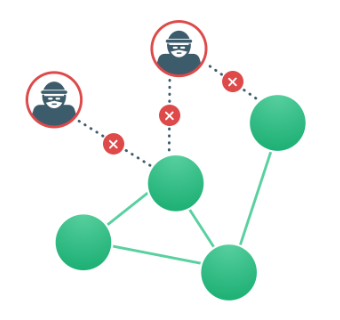
\includegraphics[width=.77\linewidth]{chapter2/privacyEsterno.png}
        \caption{Only allowed users can participate in the network}
    \end{minipage}\hfill
    \begin{minipage}{0.48\textwidth}
        \centering
        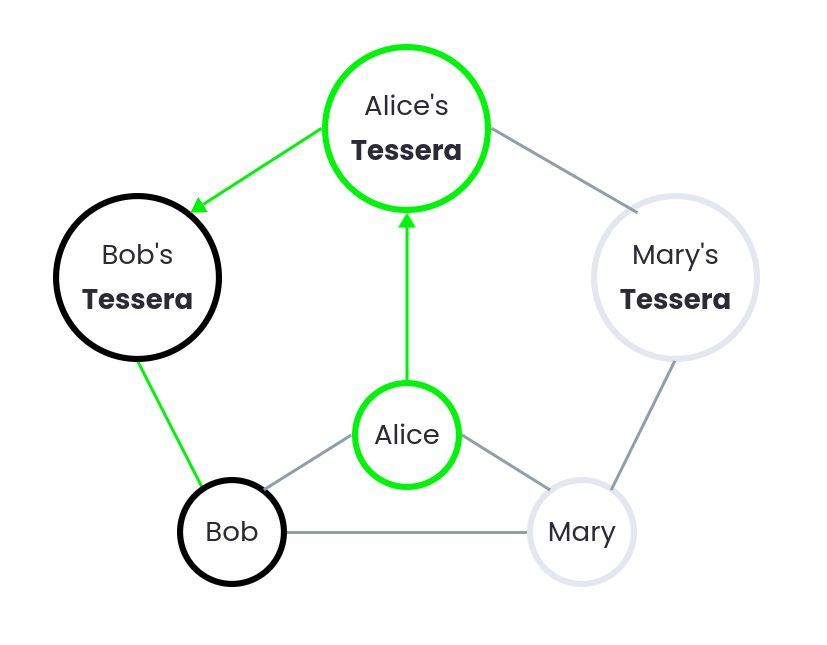
\includegraphics[width=1\linewidth]{chapter2/privacyInterno.png}
        \caption{Mary cannot see the private transaction sent from Alice to Bob}
    \end{minipage}
\end{figure}
\begin{figure}[!htb]
    \begin{minipage}{0.48\textwidth}
        \centering
        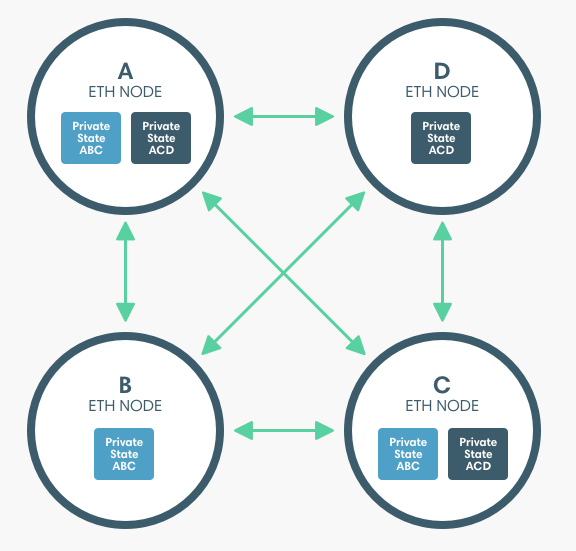
\includegraphics[width=.77\linewidth]{chapter2/privacyGroups.png}
        \caption{Restricted visibility of two Privacy Groups (light blue and blue)}
    \end{minipage}\hfill
    \begin{minipage}{0.48\textwidth}
        \centering
        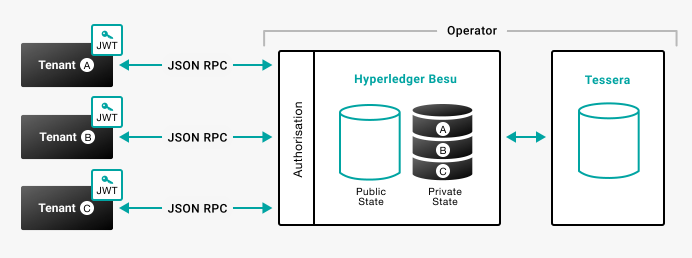
\includegraphics[width=1\linewidth]{chapter2/multiTenant.png}
        \caption{Besu and Tessera pair nodes administrator can give access to other Tenants, i.e., users.}
    \end{minipage}
\end{figure}\\
Privacy is enabled both externally to the network and internally: through private 
transactions, not all nodes can access certain information, and nodes that want to 
take advantage of private transactions must have an associated \textbf{Tessera} node, which 
will take care of the cryptographic part.\\
Even \textbf{Privacy Groups} can be created: those who do not belong to the group cannot access 
particular data. In addition, another interesting feature is that of Multi-Tenant 
management: multiple participants can use the same Besu and Tessera node through a 
dedicated user system.

\subsubsection{Hyperledger Fabric}
Hyperledger Fabric is an enterprise-grade, proven, and open distributed ledger 
platform (DLT). It provides advanced privacy controls so that only the shareable 
data is transmitted among network participants, known as "authorized".\\
It offers a modular architecture that makes available components (mechanism for 
consensus, services for joining and managing blockchain members) that can be activated
within a blockchain with plug-and-play logic. It can be said to be very similar to 
Besu (also a permissioned and privacy-oriented), with the big difference being that 
it is not EVM compatible so the smart contracts will be written in languages such as 
Java and Go instead of Solidity.
\subsection{Libraries and Stack involved}
\subsubsection{EBSI}
\subsubsection{walt.id SSI Kit}

% /*//////////////////////////////////////////////////////////////
%                        STATE OF THE ART
% //////////////////////////////////////////////////////////////*/
\section{State of the art}
